\documentclass[11pt,a4paper]{vutinfth}
\usepackage[utf8]{inputenc}
\usepackage{graphicx}
\usepackage{textcomp}
\usepackage{caption}
\usepackage{mathtools}
\usepackage{amssymb}
\usepackage[boxed,linesnumbered]{algorithm2e}
\usepackage{color}
\usepackage{subcaption}
\usepackage{amsthm}



%TODO: CHANGE!
\setauthor{}{Jakob Klinger}{}{male}
\setadvisor{Ass.Prof. Dipl.-Inform. Dr.rer.nat}{Martin Nöllenburg}{}{male}%{Pretitle}{Forename Surname}{Posttitle}{male}
\setfirstassistant{Univ.Ass.}{Fabian Klute}{ M.Sc., B.Sc.}{male}
%Ass.Prof. Dipl.-Inform. Dr.rer.nat. Martin Nöllenburg
% University Assistant, M.Sc., B.Sc. Fabian Klute

\setaddress{Scherzergasse 10/8, 1020 Wien}
\setregnumber{1125755}
\setdate{25}{09}{2017}%TODO: Update

\settitle{Boundary Labeling for annotated documents}{Boundary Labeling in annotierten Dokumenten}
\setsubtitle{}{}%{TestSubtitleENG}{TestSubtitelGER}

\setthesis{bachelor}
\setcurriculum{Bachelor's programme Software \& Information Engineering}{Bachelorstudium Software \& Information Engineering} %TODO!


\newtheorem{lemma}{Lemma}
\newtheorem{theorem}{Theorem}
\newcommand{\change}[1]{\textcolor{red}{#1}}

\begin{document}

\frontmatter
%\addtitlepage{naustrian}
\addtitlepage{english}
\addstatementpage

%\begin{danksagung*}
%\todo{Ihr Text hier.}
%\end{danksagung*}

%\begin{acknowledgements*}
%\todo{Enter your text here.}
%\end{acknowledgements*}

%\begin{kurzfassung}
%\todo{Ihr Text hier.}
%\end{kurzfassung}

%\begin{abstract}
%\todo{Enter your text here.}
%\end{abstract}

\selectlanguage{english}

\tableofcontents

\mainmatter


%TODO: Abstract: \begin{abstract}...\end{abstract}

\chapter{Introduction}
Whenever additional information needs to be inserted into an existing document without altering the original text, we can make use of annotations. They usually take the form of footnotes, which require only a minimal reference in the main text, and are used for a variety of reasons - for example, to provide additional information that would hinder the text's flow if inserted directly, or as a result of a commenting tool that is used for communication between an author and their editor.
If a more obvious connection between the text and the referenced content is required, for example when lengthy comments are added, or if a change-tracking tool is used, the reference is often placed to the side of the document and visibly connected to the part of the text it is referring to. This style of annotation is easily implemented on virtual documents, since they can be hidden on demand, however if the annotations need to be included in a printed version, there are several issues that arise regarding readability of the final product and ambiguity of text-annotation assignments.

In this thesis, we will look at ways to use Boundary Labeling for this problem, which means that all annotations will be placed somewhere outside of the text they are referencing and will be visually connected to the feature they are referencing. (See also \cite{Bekos2005}) 

The guidelines on how to create suitable labelings are as follows: the connections should be as direct as possible, no important information should be obscured, and it should be easily discernable which Label belongs where. These three criteria easily come into conflict with one another, as the text usually is very dense and leaves little space for lines in between, yet one shouldn't allow them to pass through the text, as this makes the text harder to read. 

\section{Terminology and Fundamentals} 
Boundary Labeling (or equivalent concepts) can be applied to a space with different geometry or more dimensions, but this thesis will only concern itself with two-dimensional, Euclidean space.
To easily reference important concepts, some additional terminology will be introduced as well. (See Fig.~\ref{fig:term} for a visual explanation)


\begin{figure}
 \captionsetup{justification=centering, margin=0.75cm}
 \centering
  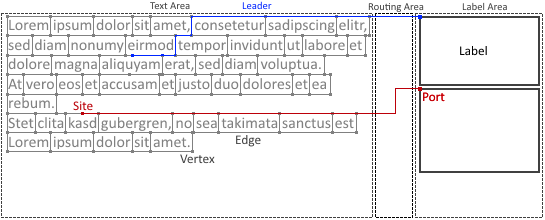
\includegraphics[scale=0.95]{GraphTerminologyExtended.png}
  \caption{Illustrated guide to the labeling terminology}
 \label{fig:term}
\end{figure}

A \emph{graph} $G=\langle V, E \rangle$ is a tuple of \emph{vertices} $V=\{v_1, v_2, ..., v_n\}$ and \emph{edges} $E=\{e_1, e_2, ..., e_m\}$. A vertex $v$ is a featureless object. %Wie  sage ich, dass die Umsetzung der Vertices sehr flexibel ist?
 Each edge $e$ is a relation between two vertices $E \subseteq V\times V$. %Edges can also be directional, or have a weight, which affects how they are treated by algorithms.
We call two vertices $u,v \in V$ \emph{adjacent}, if the edge $e=(u,v) \in E$.
 A \emph{path} $P=v_1, ..., v_h$ is an ordered sequence of vertices, where each vertex must have an edge connecting it to the subesquent one.
 \emph{Depth-first search} is a searching algorithm on a graph G that starts at a given vertex $v \in V$ and explores the graph by traversing its edges as far as possible before backtracking, and continues to do so until a pre-defined goal is met. 
%A function is called \emph{monotone} if it is either non-decreasing or non-increasing, meaning that for each $x<y$, $f(x) \leq f(y)$ for \emph{monotonically increasing functions}, or $f(x) \geq f(y)$ for \emph{monotonically decreasing} functions.


A \emph{polyline} is a sequence of points $O=p_1, p_2, ...,p_n$, connecting each point to its successor with straight lines. Each point $p \in O$ cannot be equal to any other point in $O$.
We will call a polyline $O$ \emph{monotonically increasing}, if any two vertices $p_i, p_j \in O$ satisfy the following: $\forall p_i, p_j \in O: i<j \iff (X(p_i)\leq X(p_j) \land Y(p_i)\leq Y(p_j)\land p_i \neq p_j)$, where $X(.)$ returns a point's X-coordinate, and $Y(.)$ returns its Y-coordinate.

\emph{Labels} hold additional information and are represented as boxes containing this information. They always have a \emph{port}, a special point on the label's border which will be defined later. Labels are usually placed in the \emph{label area} which is a rectangular area designated to hold labels. It is located next to of the bigger, rectangular \emph{text area}, which contains the document's text and all \emph{sites}, the points or objects that a label's information refers to. If multiple label areas exist on different sides of the text area, we speak of \emph{multi-sided labeling}, otherwise we speak of \emph{one-sided labeling}. We will be using one-sided labeling in our implementation. Some space was left in between the text and label area, to make connecting sites to their labels easier, which we will call the \emph{routing area}. The site and the label are connected via a \emph{leader}, a polyline that can be further classified by looking at the orientation of its segments: \emph{O-Segments} run orthogonally to the border of the label area. \emph{P-Segments} run parallel to the border of the label area, and as such must be combined with other segments for the leader to reach its destination. \emph{S-Segments} are not required to have any particular orientation, and simply connect their start and ending points in a straight line.
The leader's name is created by combining the name of the segments - for example, the blue leader from Fig~\ref{fig:term} would be classified as an OPOPO-Leader.
The location where a leader connects to the label is called the \emph{port}. It can be restricted to pre-defined positions. %TODO: Re-insert monotonicity


\section{Related Work}

Boundary labeling was first introduced by Bekos et al. in 2004 (see \cite{Bekos2005}), where both one-sided and multi-sided labelings with different leader types are looked into. They also showed that the optimal placement of arbitrarily-sized labels on two sides of the text area can be NP-hard by drawing comparisons to the Partition-Problem. However, a pseudo-polynomial solution exists for this problem, which was adapted to this variation of the problem.

Since then, several papers have been written about boundary labeling. One of these is \cite{Barth2015}, which looks into the readability of different leader styles. Interestingly, some leader styles perform quite well, despite the study's participants preferring others over them, with OPO-Leaders being both least preferred and the hardest to follow.

Another article using boundary labeling is \cite{Goetzelmann2006} by G{\"o}etzelmann et al., which creates boundary labeling-style annotations along other methods to label different parts of three-dimensional figures, resulting in pictures similar to what could be found in a textbook. As this algorithm works in real-time, it is suitable for labeling interactive models and allows for user interaction.


%Beispiele von suboptimalen Lösungen einfügen? (Bilder)
Boundary labeling in text documents however, is rarely discussed, and only few papers exist about this topic. The programs that employ this style of annotation often also use rather simple algorithms, to mediocre results or make extensive use of the interactivity of a digital medium, showing annotations only on demand. However, the few papers that approach this topic add interesting information to the discussion.

The paper about the Luatodonotes-Package\cite{Kindermann2014} uses several styles of drawing leaders, and came to the conclusion that leaders without bends are easier to follow, which fits with \cite{Barth2015}'s observations, which ranks OPO- and PO-Leaders lower than other variants.
However, most solutions proposed in \cite{Kindermann2014} do not consider whether a path overlaps with text or not, which results in a decrease in readability. While we do not use the routing and leader styles introduced in this paper, the results can be used in comparisons regarding readability of the main text and ease of use of the different leader styles.%Bsp-Bild einfügen!

The thesis by Loose\cite{Loose2015} on the other hand is based around only using the free space between lines and words, which produces longer leaders, and forces curves, but doesn't obscure any part of the text. The two different approaches in this paper were a clustering-based algorithm, which was previously described in \cite{Nollenburg2010}, and a flow network-based approach. Several concepts of this paper, such as the graph-based strategy and the usage of a routing area will be adopted in our thesis and it is by far the biggest influence on our approach to the problem.  %Anmerken, dass viele Konzepte hier aufgegriffen werden!

Lin et al.\cite{Lin2009} use only OPO-Leaders that have their P-Segment located outside of the text area in their paper, but allow the leaders to use the text area's border on the opposite side of the label area to route upwards or down. This allows for more labels to be placed as close as possible to their leader's source, at the cost of increasing select leaders' length and placing some labels out of order. While this is an interesting way to avoid longer leaders in general, it is hard to combine with the graph-based routing that happens inside the text area, so we won't make use of it.


\chapter{The Algorithm}
%1 Zeile Einleitung hier einfügen - zb: Kapitelübersicht
\section{Problem Specification}
\label{sec:ProbSpec}
We limited the leaders to use exclusively O- and P-Segments, and banned them from passing through words. We also place labels as far up as possible to maximize the space remaining for  remaining placements. Additionally, a leader isn't allowed to be any longer as is necessary to connect a given Site with its label's port.

These restrictions are implemented as follows: We divided the text $T=\{W,H\}$ into separate lines $L=\{l_1 ,l_2 , ... ,l_n\}$ which are in turn made up of words $w \in W$ and whitespace $h \in H$, which alternate, starting and ending with a word, which creates a sequence $l=(w_1,h_1,w_2, ... , h_{m-1},w_m)$, where $m$ is the number of words in $l$. The width of each line is equal to the text area's total width in characters $(width)$, which means that $m \leq \frac{width}{2}$. The remaining space between lines is called $S=\{s_1, ... s_{n+1}\}$, with $n$ being the number of lines in $L$. For each $l_i \in L$,  $s_i$ is the space directly above that line. All $s \in S$ are the same height and width, even $s_1$ and $s_{n+1}$, which only have lines on one of their sides. The $s \in S$ and $l \in L$ are arranged in alternating order in the text $T=\{s_1, l_1, s_2, l_2, ..., s_n, l_n, s_{n+1}\}$.  For each word $w \in W$, we define $R(w)$  as its bounding rectangle, which marks the space leaders aren't allowed to cross. For a graphical representation see Fig.~\ref{fig:wbound}.

\begin{figure}
 \centering
 \begin{subfigure}[b]{\textwidth}
 \centering
  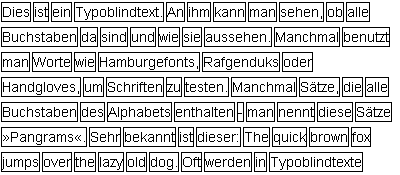
\includegraphics[]{WordBoundaries.png}
  \caption{\label{fig:wbound}}
 \end{subfigure}
 \\
 ~\\%There's probably a better way to force multiple newlines...
 \begin{subfigure}[b]{\textwidth}
 \centering
  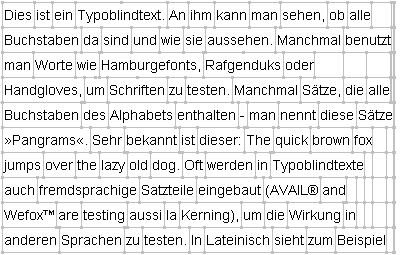
\includegraphics[]{RoutingGraph_edited.png}
  \caption{\label{fig:rgraph}}
 \end{subfigure}
 \caption{Visualization of the space reserved for the text, and the resulting graph.}
\end{figure}

Since we only allowed the Usage of O- and P-Segments in leaders, the only way for a leader to cross through a line of text is with a P-Segment through whitespace, whereas O-Segments are only usable between lines. Therefore, we can create a routing graph $G=\langle V,E\rangle$ whose Edges $E$ reflect the legal paths a leader can take within $T$.
For each line $l_i \in L$ and each whitespace character $h \in l_i$, one vertex is placed in $s_i$ and $s_{i+1}$ each, located above or below the whitespace character, and with a maximum distance from each of its neighbouring lines. The start and end of each line are also assigned a pair of vertices each. Sites will be represented by the insertion of additional vertices in $S_i$ on a similar height as those next to whitespace of the same line and located directly above the center point of its words $w_j$ bounding rectangle $R(w_j)$. The edges between the vertices are all perfectly horizontal or vertical, and do neither intersect with any bounding rectangle, nor any vertices other than their starting and ending vertex. The resulting graph looks similar to Fig.~\ref{fig:rgraph}.
In the following, we define vertex $v_a \in s_i$ to be \emph{above} another vertex $v_b \in s_j$, if $i<j$. If $v_a$ and $v_b$ are adjacent to each other, $v_a$ is \emph{directly above} $v_b$. We will also define a vertex $v_b$ to be \emph{between} two vertices $v_a$ and $v_c$, if $v_a, v_b, v_c \in s$ $(s \in S)$ and it is impossible to create a path $P \subseteq s$ using only vertices from $s$ that leads from $v_a$ to $v_c$ without including $v_b$.
Furthermore,we will call the vertices closest to the text area's border to the routing area \emph{Border Vertices} $B \subset V$. They serve as a goal for the depth-first search, and are located at the end of each line in our implementation.

Each edge has a capacity of 1, meaning that no more than one leader is allowed to pass through it. Leaders also aren't allowed to cross one another, as it is hard to discern between intersections and two leaders curving away from each other. Furthermore, they are monotonically increasing, and go as far up as possible, limited only by the previous label's placement.

The Routing Area will be used to connect each site's path with its source, using OPO-Leaders. Combined with the path $P=\{s, v_1, v_2, ..., v_h, v_b\}; P \subset V; P \cap B = v_b$ leading from the source $s \in S$ to the graph's border $(v_b \in B)$ it creates an unbroken connection between a source and its port, which shall be called a \emph{Source-Port-Path}, or \emph{SP-Path}.

\section{Description}
\label{sec:AlgDesc}

The routing algorithm works through the annotations $a \in A$ in the order they appear in the text, placing each as far up as possible, skipping any annotation that cannot be placed above its leader's source or is impossible to route. It will use fixed ports located in the top left corner of each label.

\begin{figure}
	\captionsetup{justification=centering, margin=0.75cm}
	\centering
	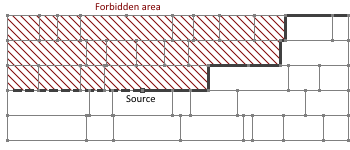
\includegraphics[scale=1]{Ceiling.png}
	\caption{Illustration of the search-space limitation by previous leaders}
	\label{fig:ceil}
\end{figure}

We use a depth-first-search algorithm with the Graph $G$ and the set of sites $V_{ann} \subset V$ as input. The Algorithm prioritizes routing to not yet visited vertices located above the current vertex and terminates either when reaching the right text border or if all possible paths failed to reach the text border, and the resulting SP-path will be monotonically increasing. If the routing for any site $v_{ann} \in V_{ann}$ failed, the algorithm returns $\bot$ for that site. \change{To ensure that routings remain crossing-free, the most recently successfully routed leader $P_last$ is used as a ceiling to the available search space. This means that any vertex above the polyline created by the vertices in $P_last$ and the connection of $P_last$'s source with the text area's border opposite of the label area is forbidden to use. (See als Fig.~\ref{fig:ceil})} This path is split into two parts: The path within the graph $(P \subset V)$, leading from the source to the text area's border, and the OPO-Leader that connects the text area's border with the Label's port. The former is implemented as a list of vertices $V_{Path} \subset V$ the leader travels through, whereas the latter is determined by the rightmost vertex of $V_{Path}$, the Port, and the location of the P-Segment. (For an illustration in Pseudocode see Alg.~\ref{alg:DFS}.)

Each SP-path's P-Segment in the Routing Area is only placed after all SP-Paths have been generated, and will be placed with equal spacing between the borders of the Routing Area and each P-segment, to ensure readability of the resulting leaders.

\begin{algorithm}

\DontPrintSemicolon
\KwData{A single annotation's source and its Graph}
\KwResult{A List of vertices describing the leader's path}

\SetKwData{G}{Graph}
\SetKwData{Path}{Path}
\SetKwData{Src}{Source}
\SetKwData{Curr}{currentVertex}
\SetKwData{Old}{oldVertex}
\SetKwData{Back}{backtracking}

\SetKwFunction{Top}{getTopNeighbourOf}
\SetKwFunction{Right}{getRightNeighbourOf}
\SetKwFunction{AddVert}{addVertex}
\SetKwFunction{RemVert}{RemoveVertex}
\SetKwFunction{Last}{getLastEntry}
\SetKwFunction{Below}{isBelow}
\SetKwFunction{Break}{break}

initialization\;
\While{\Curr not at right text border}{
 
 \uIf{$($\G.\Top{\Curr}$\neq null)\land \neg$\Back and previous Vertex not part of other leaders}{
  \Path.\AddVert{\Curr}\;
  \Curr $\gets$ \G.\Top{\Curr}\;\;
 }
 \uElseIf{\G.\Right{\Curr}$\neq null$}{
 \Path.\AddVert{\Curr}\;
  \Curr $\gets$ \G.\Top{\Curr}\;
  \Back $\gets$ False\;
 }
 \Else{
  \Back $\gets$ True\;
  \Repeat{\Curr's Position is below \Old or \Path is Empty}{
   \Old $\gets$ \Curr\;
   \Curr $\gets$ \Path.\Last{}\;
   \Path.\RemVert{\Curr}\;
  }
  \;
  \If(//No path found){\Curr not below \Old}{\Break}
 }
}
\caption{The Depth-First-Search algorithm used in the program.}
\label{alg:DFS}
\end{algorithm}



\section{Analysis and Proof}

In this section we will first analyze the computation time required to create the graph. Afterwards, we will prove the correctness of our routing algorithm, and finally we will determine the algorithm's runtime complexity.

%\begin{itemize}
% \item Computation time of graph-creation
% \item Computation time of the routing algorithm
%\end{itemize}
%~\\
%Furthermore, we will prove that:
%\begin{itemize}
%\item The algorithm generates only crossing-free routings
%\item The algorithm always returns a highest (define!) legal path
%
%NOTE: The algorithm keeps the annnotations in reading order
%\end{itemize}
%~\\
\begin{lemma}
	The creation of the routing graph is in O(n).
	\label{lem:GraphCreat}
\end{lemma}

\begin{proof}
	As discussed in Section~\ref{sec:ProbSpec}, each line holds at most $\frac{width}{2}$ words, with an appropriate amount of whitespace in between. Since $width$ is a constant value, the amount of vertices placed is only dependent on the number of lines in the text, therefore $|V|=O(n)$.
	Similarly, each vertex has at most 4 incident edges, representing the two possible placements of P- or O-Segments starting from that vertex, respectively. Therefore, $|E|=O(n)$. As both the creation of new vertices and edges can be done in a constant amount of time, the overall computation time is in $O(n)$.
\end{proof}

%As discussed in section~\ref{sec:ProbSpec}, we will be placing a pair of vertices per whitespace character, as well as one additional pair at both the start and end of each line, which amounts to $2\times|H|+4\times|L|$ vertices total. Together with the sites $I$, which are also represented as vertices, this results in the total number of vertices $|V|=|I|+2\times|H|+4\times|L|$. Additionally, each vertex in a pair is connected to its counterpart, which creates $(|V|-|I|)/2$ edges, representing all possible P-Segments. Finally, each edge placed in a space $s \in S$ above or below a line will be connected to each other, which is solved by connecting each vertex to the next unconnected vertex remaining in $s$. This leads to the creation of $|s|-1$ edges representing possible P-segments, which leads to a total of $|V|-|S|$ additional edges, making the total number of edges $|E|=(3\times|V|-2\times|S|-|I|)/2$.
%If we assume that the creation of edges and vertices both take a similar amount of time, we are looking at roughly $5/2 \times |V|$ operations, which means that the algorithm scales linearly with the amount of vertices placed, which in turn is directly proportional to the number of words $|W|$ in the text.
For a representation of the graph-generation algorithm in pseudocode, see Alg.~\ref{alg:GraphCreation}.


\begin{algorithm}
\DontPrintSemicolon
\SetKwData{Words}{words}
\SetKwData{PrevW}{previousWord}
\SetKwData{G}{Graph}
\SetKwData{W}{w} \SetKwData{V}{v}\SetKwData{Va}{v1} \SetKwData{Vb}{v2}
\SetKwData{Up}{UpperVerticesList}
\SetKwData{Low}{LowerVerticesList}

\SetKwFunction{setAnn}{setAnnotation}
\SetKwFunction{NewVert}{new Vertex}
\SetKwFunction{AddVert}{addVertex}
\SetKwFunction{AddAll}{addAll}
\SetKwFunction{CEdge}{createEdgeBetween}
\SetKwFunction{PosConn}{connectBasedOnPosition}
\SetKwFunction{ClrList}{emptyList}
\SetKwFunction{getC}{getCenter}
\SetKwFunction{tLeft}{getTopLeft}
\SetKwFunction{tRight}{getTopRight}
\SetKwFunction{bLeft}{getBottomLeft}
\SetKwFunction{bRight}{getBottomRight}
\SetKwFunction{Newline}{startNewLine}

\KwData{A text with annotations,stored as a String-Array}
\KwResult{A Graph (as described above)}

 initialization\;
 
 \ForEach{\W in \Words}{
  \eIf{\W is annotation}{
   \V$\gets$\NewVert{\PrevW.\getC{}}\;
   \V.\setAnn{\W}\;
   \G.\AddVert{\V}\;
   \Up.\AddVert{\V}\;
  }{
   \If{\W is too big for the line}{
    //Create last pair of vertices in current line\;
    \Va $\gets$\NewVert{\PrevW.\tRight{}}\;
    \Vb $\gets$\NewVert{\PrevW.\bRight{}}\;
    \G.\AddAll{\Va,\Vb}\;
    \Up.\AddVert{\Va}\;
    \Low.\AddVert{\Vb}\;
    \G.\CEdge{\Va,\Vb}\;
    \;
    //Start new line\;
    \Newline{}\;
    \PosConn{\Up}\;
    \Up$\gets$\Low\;
    \ClrList{\Low}\;
   }
   \Va $\gets$\NewVert{\W.\tLeft{}}\;
   \Vb $\gets$\NewVert{\W.\bLeft{}}\;
   \;
   \G.\AddAll{\Va,\Vb}\;
   \Up.\AddVert{\Va}\;
   \Low.\AddVert{\Vb}\;
   \G.\CEdge{\Va,\Vb}\;
  }
 } 
\caption{Representation of the Graph-creation algorithm in pseudocode}
\label{alg:GraphCreation}
\end{algorithm}

%Next, we shall inspect the routing algorithm - since we use depth-first search, which is a well-known algorithm, the worst-case computation time is known to be $|V|+|E|$. As both $|V|$ and $|E|$ are in $O(n)$, so is our routing algorithm.

%To reach this time, we'd have to try and use every single edge in the graph, reaching each of the graph's vertices in the process. However, as our algorithm can't use any edges leading away from its target, our search space is reduced to only the vertices either in lower-numbered $s \in S$ (those ``above'' the current position) or those in the same $s$, but located between the source and the border vertices. If we also take into account that leaders aren't allowed to cross one another, this further limits our search space, removing all vertices above the previous leader's vertices.

\begin{lemma}
	The algorithm only creates crossing-free routings.
	\label{lem:CrosFree}
\end{lemma}
\begin{proof}
	As stated in Section~\ref{sec:AlgDesc}, we are forbidden to use any vertices above \change{the polyline created by the last successfully routed leader $(P_{last})$ and the direct connection of $P_{last}$'s source and the left text area's border. As this makes it impossible to construct a route that incorporates any vertex above or to the left of $P_{last}$, those two leaders cannot possibly cross each other. This is true for any two consecutive leaders, therefore each leader also cannot cross any of the leaders routed before $P_{last}$, as those are located on the other side of $P_{last}$, which contains only forbidden vertices.
	Therefore, our algorithm produces crossing-free routings.}
\end{proof}

\change{For the next part, we first need to define what we consider a \emph{highest legal path}: A \emph{legal path} is one that satisfies both the constraints of monotonicity and being crossing-free, whereas a \emph{highest path} reaches the highest possible border vertex reachable from a given source.} 

\begin{lemma}
	Our algorithm only returns a highest legal path.
	\label{lem:High}
\end{lemma}
\begin{proof}
	The legality of any generated path is given, due to the algorithm only returning monotonically increasing paths, and Lemma~\ref{lem:CrosFree}. To show that there are no reachable border vertices above the path's highest reachable border vertex $b_{high}$, we will assume there exists a vertex $b_{top} \in B$ that is located above $b_{high}$ and legally reachable via the path $P_{top}$. As the algorithm prioritizes routing to vertices directly above, the only way for the path to $b_{top}$ to reach higher vertices than $b_{high}$ would be that either $P_{top}$ would generate crossings with previously routed leaders or violate the the monotonicity constraint, which both render $P_{top}$ illegal. Since we also cannot include more than one border vertex in our path, we conclude that such a path cannot exist.
\end{proof}

\begin{theorem}
	The routing problem can be solved with a worst-case time complexity of $O(n^2)$ for all sources.
\end{theorem}
\begin{proof}
	As part of the proof for Lemma~\ref{lem:GraphCreat}, we have shown that the total number of vertices $|V|$ is in $O(n)$. Since $S \subset V$, $|S|$ must too be in $O(n)$. 
	We have proven our algorithm's solutions to be correct in the Lemmas \ref{lem:CrosFree} and \ref{lem:High}.
	The performance of our routing algorithm is easily calculated, as depth-first-search has a worst-case-performance of $|V|+|E|$, which is in $O(n)$ for our problem, as $|E|$ is in $O(n)$ as well. (See Lemma~\ref{lem:GraphCreat})
	Therefore, our overall computation time comes out to $|S| \times O(n)$, or $O(n^2)$.
\end{proof}




%First, we create the graph that will be used for the routing part of the algorithm. To achieve this, we go through the annotated text word by word in reading order, and measure the length $le(w_i)$ of each word $w_i$ that is not part of an annotation to determine its placement in the text.  At this point, we can also assign a line $l_j$ to it. Afterwards, we create new vertices above and below the whitespace characters $h_k, h_{k+1}$ preceding and succeeding $w_i$. These vertices are located in the space $s_j, s_{j+1}$ between the word's line and its surrounding lines $l_{j-1}$ and $l_{j+1}$, as described in the previous section. Whenever an annotation is encountered, a single vertex is added above the last non-annotation word in $s_j$ at $pos(h_k)+le(w_i)/2$.
%For a representation of this process in pseudocode, see Alg.~\ref{alg:GraphCreation}.
%To create leaders that exclusively use the space not taken up by a word's bounding rectangle, we decided to use a graph similar to the one Loose \cite{Loose2015} used.
%As each vertex represents a physical location, they will have co-ordinates associated with them, and the vertices representing the sites will hold additional information regarding its leader and label. 
%The graph is constructed by placing vertices between the lines, located next to each corner of a word's bounding rectangle, with two consecutive words in a line sharing the two vertices associated with their adjacent corners. 
%For the sites, we inserted an additional vertex above the center of the word, which will serve as the leader's starting point. After placing all vertices, we created edges between each vertex and the closest horizontal neighbour to both sides, and between nodes that are located exactly above or below each other, and exactly one line apart. (For a representation in Pseudocode, see Alg.~\ref{alg:GraphCreation})


\chapter{Implementation}
The program was written in Java 1.8.0u40, using JGraphT1.0.1\cite{JGraphT} as graph library. Since we only want to create leaders that don't intersect with the text, the graph was created alongside the placement of the words on the canvas.%, as it was easy to extract measurements at this point. Due to some problems with Java's various methods of calculating linebreaks, this process was done completely by hand.
\section{Challenges}

%As the Graph's vertices represent fixed locations on the canvas, they each have coordinates associated with them, with the vertices representing the sites containing extra information, such as references to the corresponding annotation and to the leader connecting the two (if existent).
%The additional information stored in the vertices is used for both routing and drawing the leaders: The routing was done via a depth-first search algorithm that prioritized vertices located further up if possible, and vertices to the right otherwise. After the algorithm terminates, it returns  a vertex-based graph walk describing the route from the site to the border of the text area alongside information about where to draw the OPO-segment in the buffer zone if successful, or a walk containing only the starting vertex, if no valid path was found. Using this information alongside the positional data stored in the vertices, the polyline representing the leader can be drawn.


%TODO: Schönheitsfeatures, etc.
%TODO: Code genauer durchlesen und erweitern!



% For demonstration purposes, we also included another algorithm that uses S-Leaders for this section.

\chapter{Evaluation and Testing}

\section{Data generation} %(Bin mit dem Titel unzufrieden, aber hier soll beschrieben werden, wie ich die einzelnen Testfälle erstellt habe.)

\section{Testing methods}

\section{Results}

\chapter{Conclusion}

\section{Further notes}



%Section Ideas: The Program/Framework (Modellerklärung), The Algorithm(s), Implementation, Evaluation, Conclusion


\backmatter %TODO: Es gibt mehr nützliche Kommandos in VUTINFTH für zb Listen von Bildern, etc.!

\bibliographystyle{plain}
\bibliography{references}

\end{document}